\documentclass{article}
\usepackage[landscape]{geometry}
\usepackage{url}
\usepackage{multicol}
\usepackage{amsmath}
\usepackage{esint}
\usepackage{amsfonts}
\usepackage{tikz}
\usetikzlibrary{decorations.pathmorphing}
\usepackage{amssymb}
\usepackage{graphicx}
\usepackage{float}
\usepackage{colortbl}
\usepackage{xcolor}
\usepackage{mathtools}
\usepackage{enumitem}
\usepackage[symbol]{footmisc}
\makeatletter

\newcommand*\bigcdot{\mathpalette\bigcdot@{.5}}
\newcommand*\bigcdot@[2]{\mathbin{\vcenter{\hbox{\scalebox{#2}{$\m@th#1\bullet$}}}}}
\renewcommand{\thempfootnote}{\fnsymbol{mpfootnote}}
\makeatother

\title{Unit 1 - Structure and Properties}
\usepackage[T1]{fontenc}
\usepackage[utf8]{inputenc}
\usepackage[english]{babel}

\advance\topmargin-.8in
\advance\textheight3in
\advance\textwidth3in
\advance\oddsidemargin-1.5in
\advance\evensidemargin-1.5in
\parindent0pt
\parskip2pt
\newcommand{\hr}{\centerline{\rule{3.5in}{1pt}}}
%\colorbox[HTML]{e4e4e4}{\makebox[\textwidth-2\fboxsep][l]{texto}
\begin{document}

\begin{center}{\huge{\textbf{Unit 1 - Structure and Properties}}}\\
\end{center}
\begin{multicols*}{3}

\tikzstyle{mybox} = [draw=black, fill=white, very thick,
    rectangle, rounded corners, inner sep=10pt, inner ysep=10pt]
\tikzstyle{fancytitle} =[fill=black, text=white, font=\bfseries]

%------------ Quantum Theory ---------------
\begin{tikzpicture}
\node [mybox] (box){%
    \begin{minipage}{0.3\textwidth}
    \textbf{Bohr-Rutherford Model (1913)}: in this atomic model, presented by Niels Bohr and Ernest Rutherford, electrons orbit around a small, dense nucleus. \\
    \textbf{Electromagnetic Radiation}: perpendicular electric and magnetic fields moving through space as waves. \\ \\
    $\displaystyle{\lambda=\frac{c}{\nu}}$ and $\displaystyle{E=h\nu}$
    \begin{itemize}
        \item $\lambda$ = wavelength (m)
	\item $\nu$ = frequency (Hz)
	\item $c$ = speed of light in vacuum ($2.998\times10^{8}\,ms^{-1}$)
	\item $E$ = energy of light in Joules (J)
	\item $h$ = Planck's constant ($6.626\times10^{-34}\,J\cdot{s}$)
    \end{itemize}
    $\star$ The \textbf{quantum mechanical model of the atom} treats the electron like a wave.
    \end{minipage}
};
%------------ Quantum Theory Header ---------------------
\node[fancytitle, right=10pt] at (box.north west) {Quantum Theory};
\end{tikzpicture}

%------------ Atomic Spectra ---------------
\begin{tikzpicture}
\node [mybox] (box){%
    \begin{minipage}{0.3\textwidth}
    \textbf{Photon}: a packet of electromagnetic energy. \\
    \textbf{Quantum}: an indivisible packet of energy that must be absorbed or emitted in an ``all or none'' manner. \\
    \textbf{Emission Spectrum} or \textbf{Line Spectrum}: atoms of a specific element emit a series of separate lines of different colours as their excitation energy decreases.
    \begin{itemize}
        \item atoms emit/absorb particular colours of light
	\item the frequencies emitted/absorbed are the same
	\item an emission spectrum is formed when electricity is run through an element in gas form
	\item an absorption spectrum is formed when light is shone through a gaseous element
	\item sunlight produces a \textit{continuous spectrum}, which contains all the wavelengths in the visible region of the electromagnetic spectrum
    \end{itemize}
    Bohr used the line spectrum of hydrogen when it was ``excited'' to discover the energies of each energy level in the hydrogen atom.
    \end{minipage}
};
%------------ Atomic Spectra Header ---------------------
\node[fancytitle, right=10pt] at (box.north west) {Atomic Spectra};
\end{tikzpicture}

%------------ Electron Transitions ---------------
\begin{tikzpicture}
\node [mybox] (box){%
    \begin{minipage}{0.3\textwidth}
    \textbf{Ground State}: the orbit that has the lowest possible energy of the atom. \\
    \textbf{Excited State}: when an atom absorbs energy. \\
    An atom can become excited in one of two ways:
    \begin{enumerate}
        \item collide with a highly energetic particle like an $e^{-}$ in an electric current passing through a gas.
	\item absorb a photon where its energy is equal to the difference between the energy of the orbit it occupies and the energy of a higher orbit.
    \end{enumerate}
    Used to calculate the potential energy of an electron in a hydrogen atom. Calculating $\Delta E$ determines the energy of a photon required to cause a transition. \\ \\
    $\displaystyle{E_{n}=-\frac{2.18\times 10^{-18}J}{n^{2}}}$, $\Delta E=E\textsubscript{higher}-E\textsubscript{lower}$ \\ \\
    The Rydberg formula calculates the wavelength of light emitted from a specific electron transition in hydrogen-like elements (only 1 electron). \\ \\
    $\displaystyle{\frac{1}{\lambda}=RZ^{2}\left(\frac{1}{n_{l}^{2}}-\frac{1}{n_{u}^{2}}\right)}$
    \begin{itemize}
        \item $R$ = Rydberg constant ($1.097\times 10^{7}\,m^{-1}$)
        \item $Z$ = atomic number and $n$ = energy level
    \end{itemize}
    \end{minipage}
};
%------------ Electron Transitions Header ---------------------
\node[fancytitle, right=10pt] at (box.north west) {Electron Transitions};
\end{tikzpicture}

%------------ Orbitals ---------------
\begin{tikzpicture}
\node [mybox] (box){%
    \begin{minipage}{0.3\textwidth}
    \textbf{Atomic Orbital}: a region in space around the nucleus that is related to a specific wave function.
    \begin{itemize}
        \item they are three-dimensional
	\item they contain a maximum of two electrons
	\item shapes are predicted by Schröndinger's equation
    \end{itemize}
    The \textbf{orbital-shape quantum number, l}, is used to describe an orbital's shape. \\ \\
    \begin{tabular}{| c | c | c | c | c | c |}
	\hline
        Value of l & 0 & 1 & 2 & 3 & 4 \\ \hline
        Name of orbital & s & p & d & f & g \\
	\hline
    \end{tabular} \\ \\
    $\star$ The \textit{overall shape} of an atom is a combination of all its orbitals.
    \end{minipage}
};
%------------ Orbitals Header ---------------------
\node[fancytitle, right=10pt] at (box.north west) {Orbitals};
\end{tikzpicture}

%------------ Quantum Numbers ---------------
\begin{tikzpicture}
\node [mybox] (box){%
    \begin{minipage}{0.3\textwidth}
    \textbf{Quantum Numbers}: integers that describe specific properties of electrons in atoms, arising from the solutions to the wave equation. \\
    \textbf{The Principle Quantum Number, n}: indicates the energy level and relative size of an atomic orbital. \\
    $\rightarrow$ The value of $n$ can range from $n$ = 1 to $n$ = $\infty$. \\
    $\rightarrow$ The differences between energy levels become smaller as $n$ gets larger. \\
    \textbf{The Orbital-Shape Quantum Number, l}: describes the shape of atomic orbitals within each principle energy level, it refers to energy \textbf{sublevels}. \\
    $\rightarrow$ The values of $l$ are dependent on the value of the principle quantum number, $n$. \\
    $\rightarrow$ The values of $l$ are positive integers that range in value from 0 to ($n-1$). \\
    $\rightarrow$ The number of possible values for $l$ in a given energy level is the same as the value of $n$. \\
    \textbf{Zeeman effect}: the splitting of the spectral lines of an atom in the presence of a strong magnetic field. \\
    \textbf{The Magnetic Quantum Number, $\mathbf{m_{l}}$}: indicates the orientation of the orbital in the space around the nucleus. \\
    $\rightarrow$ The value of $m_{l}$ depends on the value of $l$. \\
    e.g. $p$ orbitals have the same shape and energy for a given value of $n$, but different orientations around the nucleus which are designated $p_{x}$, $p_{y}$, and $p_{z}$. \\
    $\rightarrow$ For any given value of $l$, there are ($2l+1$) values for $m_{l}$ ranging from $-l$ to $+l$. \\
    e.g. If $l$ = 1, $m_{l}$ can be -1, 0, or +1. \\
    \textbf{The Spin Quantum Number, $\mathbf{m_{s}}$}: specifies the orientation of the axis on which the electron is spinning. \\
    $\rightarrow$ Has only two possible values: $\displaystyle{+\frac{1}{2}}$ or $\displaystyle{-\frac{1}{2}}$. \\
    Quantum Numbers for Helium: \\
    \def\arraystretch{1.5}
    \begin{tabular}{| c | c |}
	\hline
        Electron & Quantum Numbers \\ \hline
        First & $n$ = 1, $l$ = 0, $m_{l}$ = 0, $m_{s}$ = $+\frac{1}{2}$ \\ \hline
        Second & $n$ = 1, $l$ = 0, $m_{l}$ = 0, $m_{s}$ = $-\frac{1}{2}$ \\
	\hline
    \end{tabular} \\ \\
    $\rightarrow$ The total number of orbitals for any energy level $n$ is given by $n^{2}$. \\
    $\rightarrow$ In general, in any energy level, $n$, there can be no more than $2n^{2}$ electrons.
    \end{minipage}
};
%------------ Quantum Numbers Header ---------------------
\node[fancytitle, right=10pt] at (box.north west) {Quantum Numbers};
\end{tikzpicture}

%------------ Electron Configurations ---------------
\begin{tikzpicture}
\node [mybox] (box){%
    \begin{minipage}{0.3\textwidth}
    \textbf{Pauli Exclusion Principle}: a maximum of two electrons can occupy an orbital, and the electrons must have opposite spins. \\
    $\hookrightarrow$ No two electrons in an atom can have the same four quantum numbers. \\
    \textbf{Aufbau Principle}: each electron occupies the lowest energy orbital available. \\
    $1s<2s<2p<3s<3p<4s<3d<4p<5s<\dots$ \\
    \textbf{Hund's Rule}: single electrons with the same spin must occupy each equal-energy orbital before additional electrons with opposite spins can occupy the same orbitals.
    \begin{figure}[H]
        \centering
        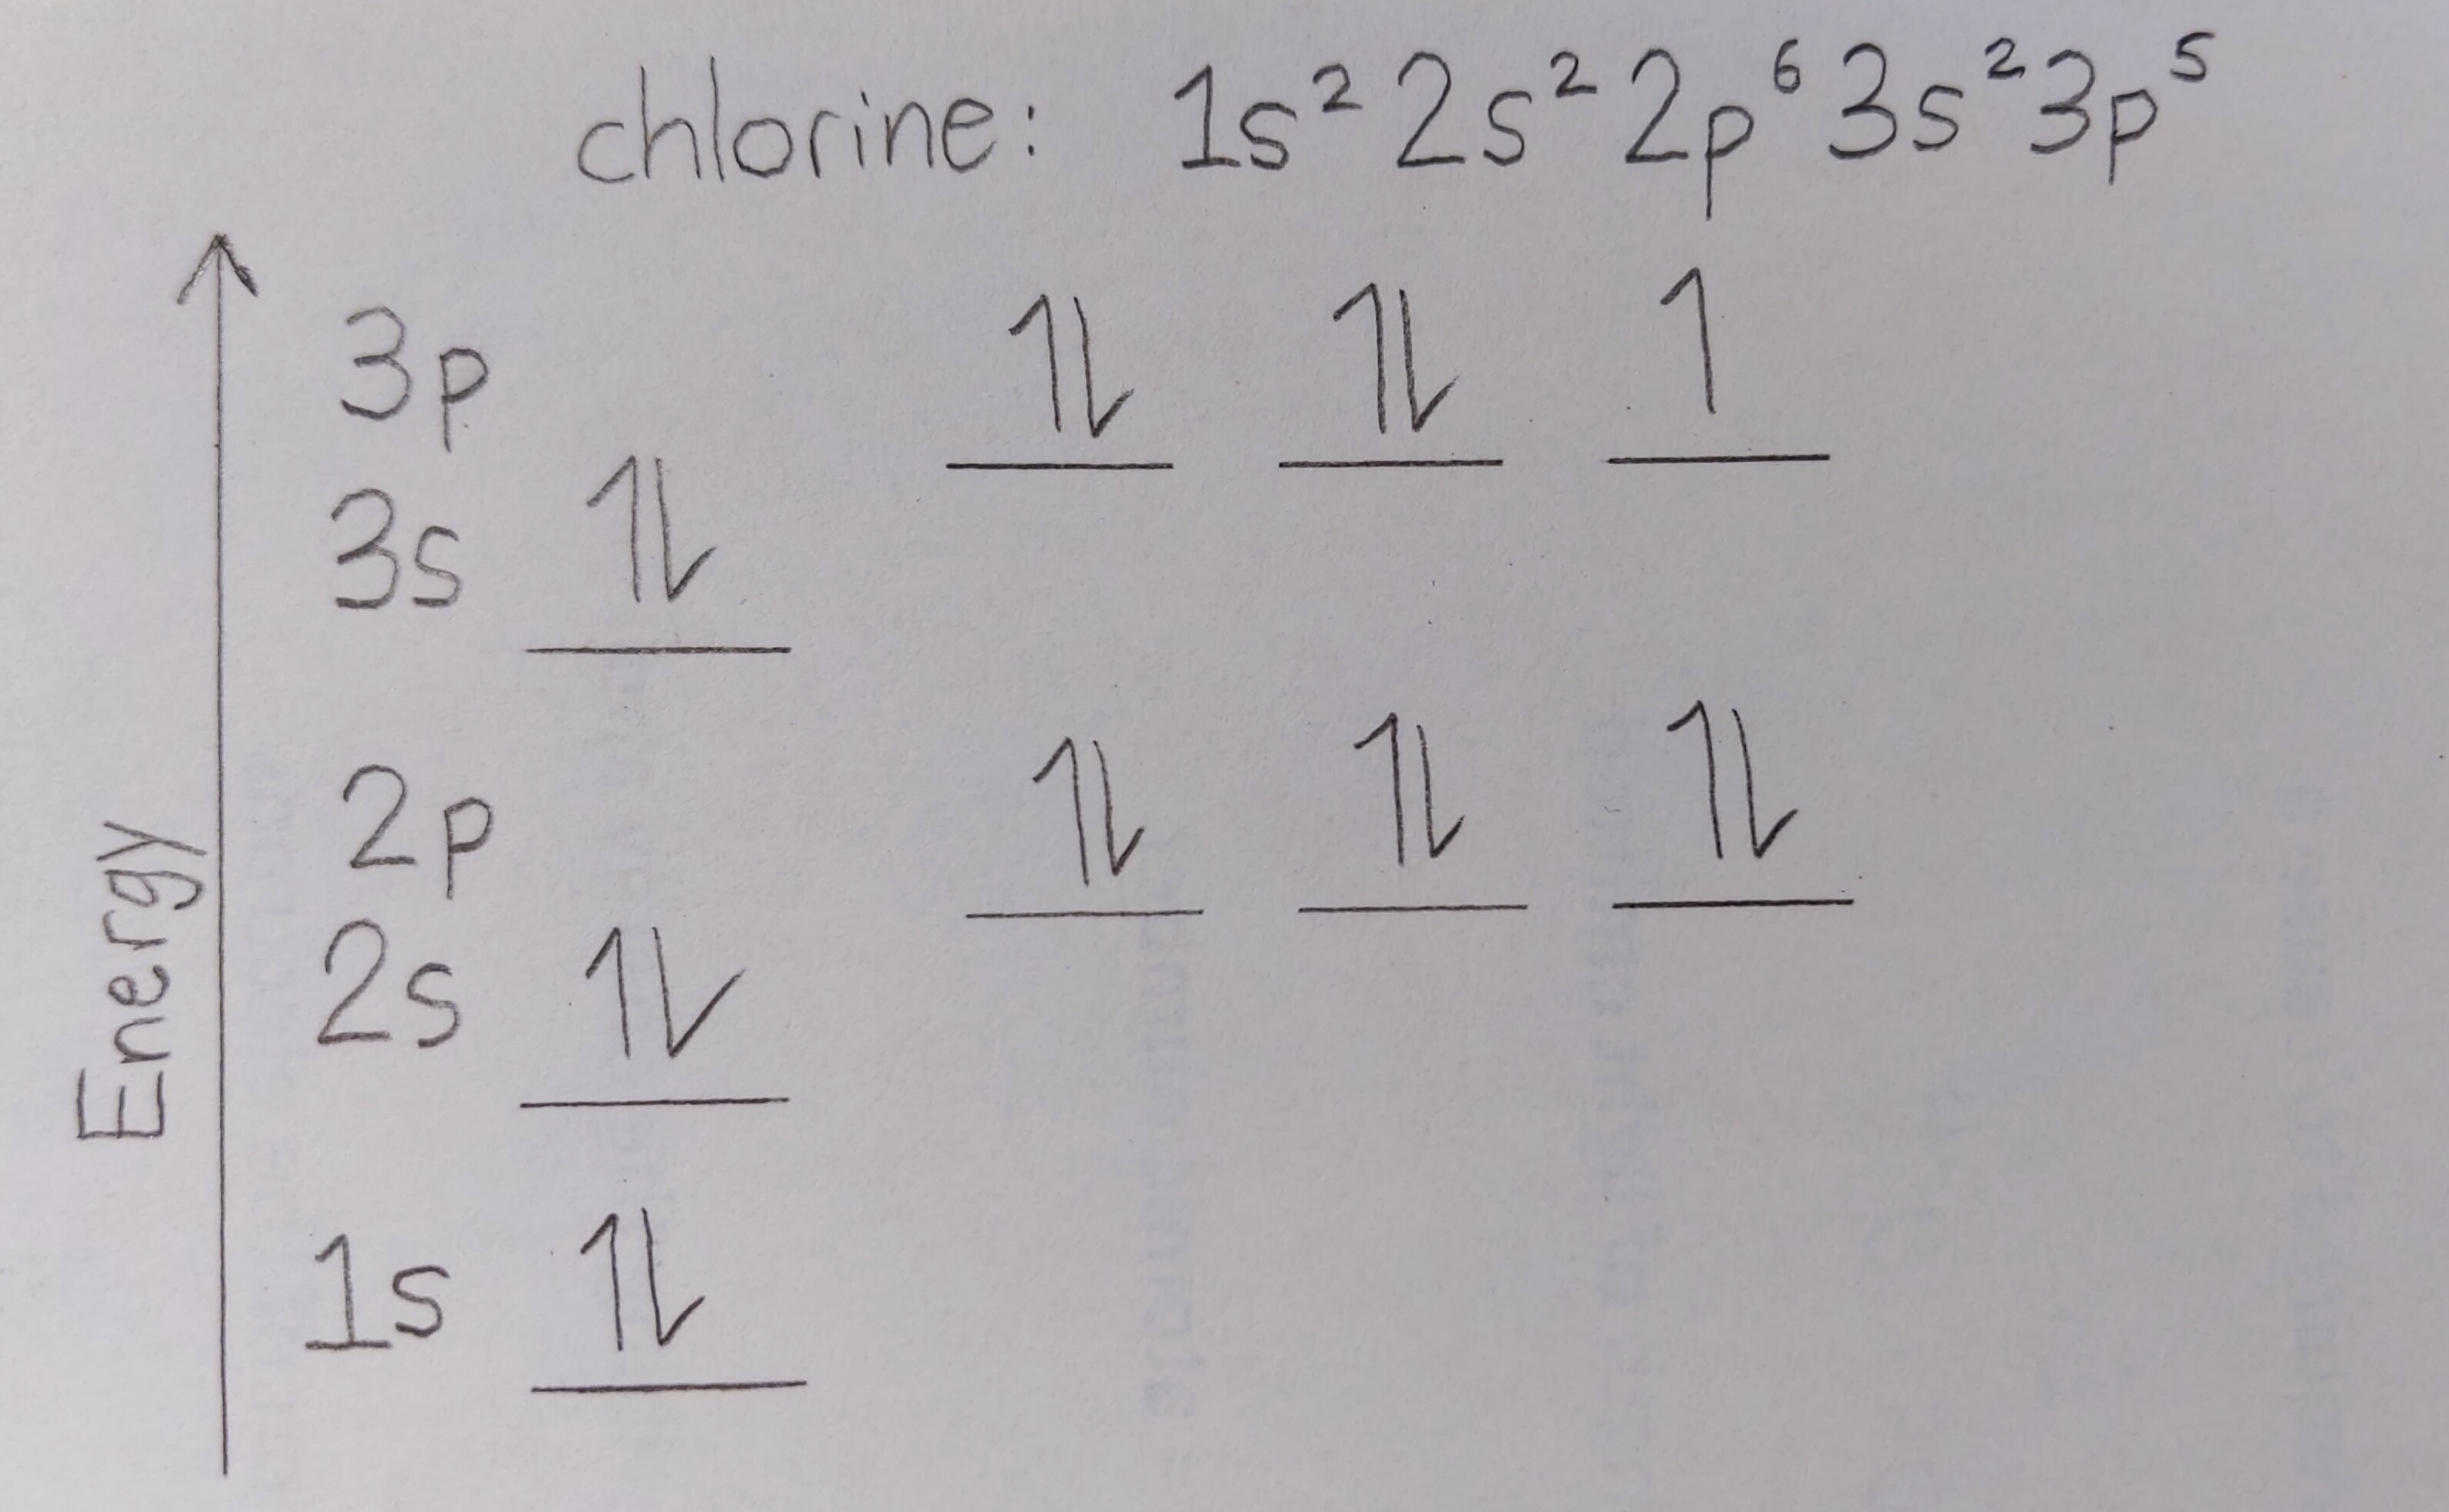
\includegraphics[scale=0.05]{diagrams/energy-level.jpg}
        \label{fig:energy}
    \end{figure}
    \textbf{Anomalous Electron Configurations} \\
    chromium: [Ar]$4s^{1}3d^{5}$, copper: [Ar]$4s^{1}3d^{10}$
    \begin{itemize}
        \item they are more stable when all of the $d$ orbitals are half-filled, than if the $s$ orbitals were filled
        \item $s$ orbitals overlap in space with nearby $d$ orbitals
        \item repulsion between electrons is minimized when electrons are removed from the $s$ orbitals first
    \end{itemize}
    \end{minipage}
};
%------------ Electron Configurations Header ---------------------
\node[fancytitle, right=10pt] at (box.north west) {Electron Configurations};
\end{tikzpicture}

%------------ Lewis Structures ---------------
\begin{tikzpicture}
\node [mybox] (box){%
    \begin{minipage}{0.3\textwidth}
    $S$, $P$, $Si$, $Cl$, and $Xe$ can have expanded octets. \\
    $\text{F.C.}=\text{\# of valence $e^-$}-\text{\# of dots}-\text{\# of lines}$
    \begin{figure}[H]
        \centering
        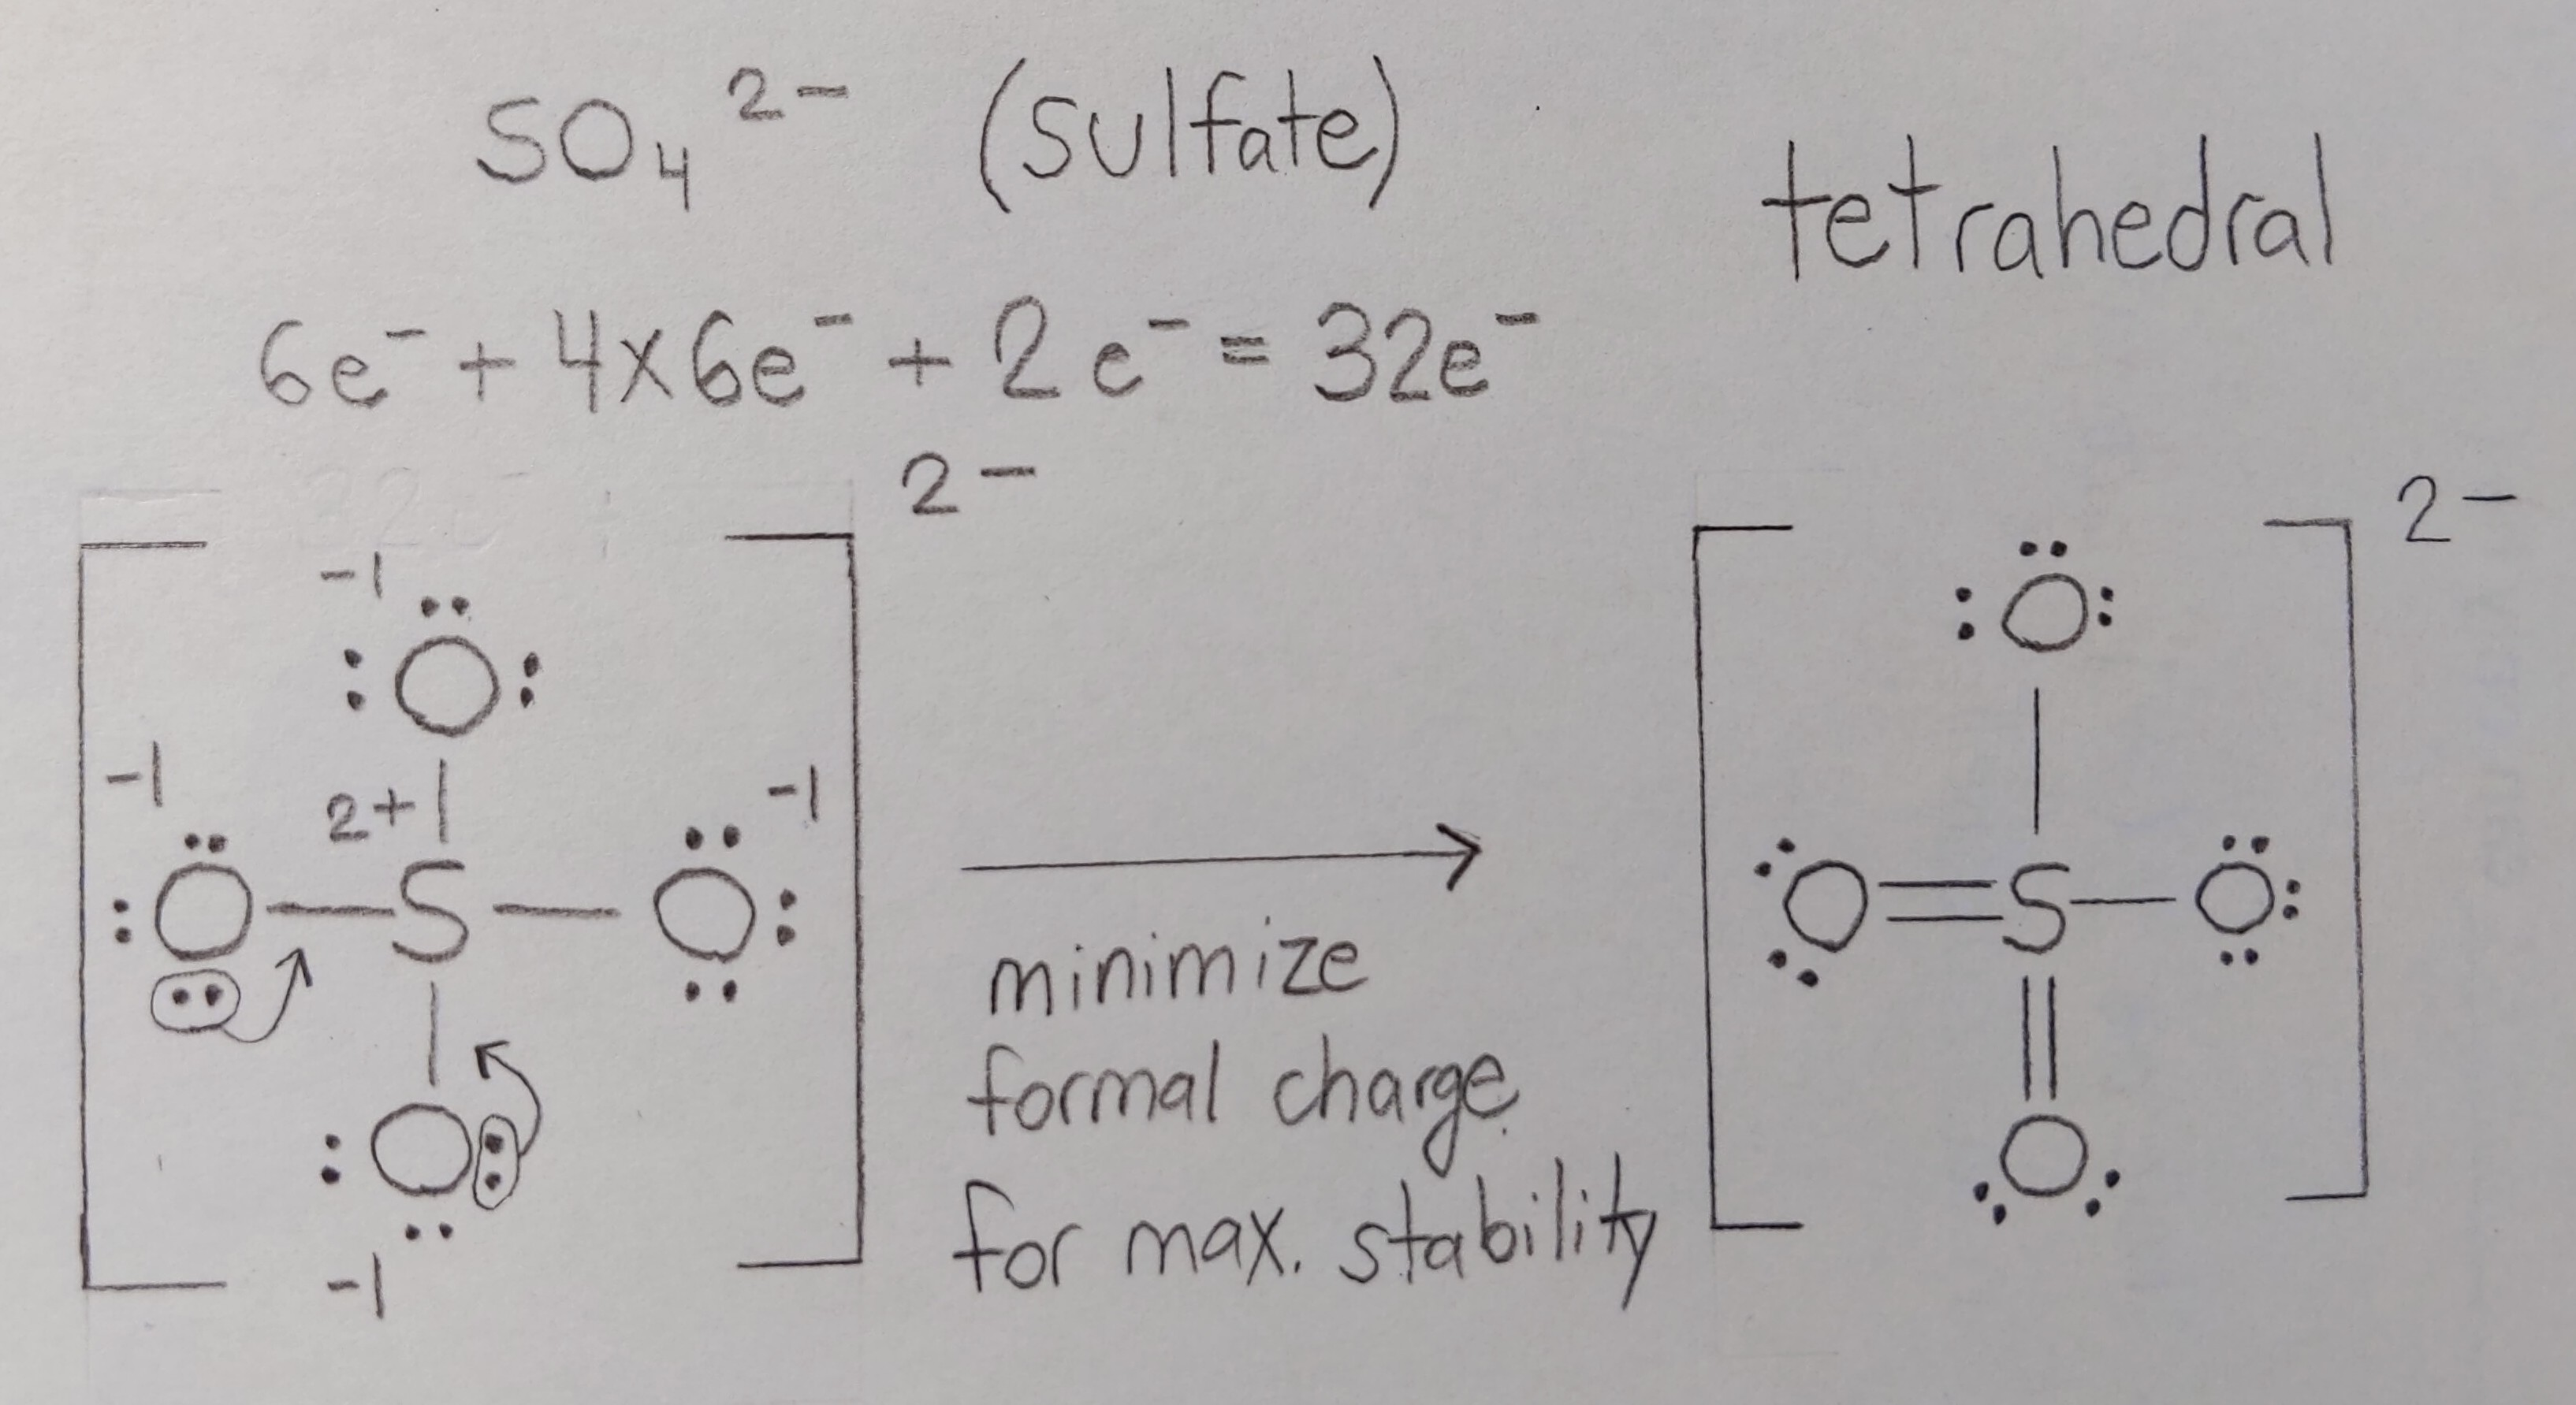
\includegraphics[scale=0.065]{diagrams/lewis-structure.jpg}
        \label{fig:lewis}
    \end{figure}
    \end{minipage}
};
%------------ Lewis Structures Header ---------------------
\node[fancytitle, right=10pt] at (box.north west) {Lewis Structures};
\end{tikzpicture}

%------------ Ionization Energy ---------------
\begin{tikzpicture}
\node [mybox] (box){%
    \begin{minipage}{0.3\textwidth}
    \textbf{Ionization Energy}: the energy required to remove an electron from a ground-state gaseous atom. \\
    The \textit{second ionization energy} is always greater than the first ionization energy. \\
    $\rightarrow$ Within a group, first ionization energies generally decrease as you move down a group. \\
    $\hookrightarrow$ Atomic radii increases, the distance of valence $e^{-}$ from the nucleus increases.\\
    $\rightarrow$ Within a period, first ionization energies generally increase from left to right. \\
    $\hookrightarrow$ Atomic radii decreases because Z\textsubscript{eff} increases.\\
    $Z\textsubscript{eff}=\text{\# of $p^+$ in the nucleus}-\text{\# of inner-shell $e^-$}$ \\
    $\star$ The repulsion of electrons in an orbital decreases the amount of energy needed to remove the electron.
    \end{minipage}
};
%------------ Ionization Energy Header ---------------------
\node[fancytitle, right=10pt] at (box.north west) {Ionization Energy};
\end{tikzpicture}

%------------ Magnetism ---------------
\begin{tikzpicture}
\node [mybox] (box){%
    \begin{minipage}{0.3\textwidth}
    \textbf{Paramagnetism}: certain materials can become magnetic when in the presence of a magnetic field. \\
    e.g. $L$, $O$, $Na$, $Al$ \\
    A material is magnetic when:
    \begin{itemize}
        \item unpaired electrons are present in its valence shell
        \item magnetic dipole moments of atoms are aligned with one another
    \end{itemize}
    When there is no external magnetic field, the magnetic fields of atoms are misaligned and cancel. \\
    \textbf{Ferromagnetism}: when tightly-packed atoms cannot misalign when the external field is taken away. \\
    e.g. $Fe$, $Ni$, $Co$, and their alloys
    \end{minipage}
};
%------------ Magnetism Header ---------------------
\node[fancytitle, right=10pt] at (box.north west) {Magnetism};
\end{tikzpicture}

%------------ VSEPR Theory ---------------
\begin{tikzpicture}
\node [mybox] (box){%
    \begin{minipage}{0.3\textwidth}
    \textbf{Valence-Shell Electron-Pair Repulsion Theory}: electron groups around an atom are positioned as far as possible from the others to minimize repulsions. \\
    An \textit{electron group} is a single bond, double bond, triple bond, or lone pair. \\ \\
    \def\arraystretch{1}
    \begin{tabular}{| c | c | c | c | c |}
	\hline
	AX & linear & H\textsubscript{2} & $s$ & 180\textdegree \\ \hline
	AX\textsubscript{2} & linear & CO\textsubscript{2} & $sp$ & 180\textdegree \\ \hline
	AX\textsubscript{3} & trigonal planar & BF\textsubscript{3} & $sp^{2}$ & 120\textdegree \\ \hline
	AX\textsubscript{4} & tetrahedral & CH\textsubscript{4} & $sp^{3}$ & 109.5\textdegree \\ \hline
	AX\textsubscript{5} & trigonal & PCl\textsubscript{5} & $sp^{3}d$ & 90\textdegree and \\
        & bipyramidal & & & 120\textdegree \\ \hline
        AX\textsubscript{6} & octahedral & SF\textsubscript{6} & $sp^{3}d^{2}$ & 90\textdegree \\
	\hline
    \end{tabular}
    \end{minipage}
};
%------------ VSEPR Theory Header ---------------------
\node[fancytitle, right=10pt] at (box.north west) {VSEPR Theory};
\end{tikzpicture}

%------------ Quantum Mechanics and Bonding ---------------
\begin{tikzpicture}
\node [mybox] (box){%
    \begin{minipage}{0.3\textwidth}
    \textbf{Valence Bond Theory}: a covalent bond forms when the atomic orbitals of two atoms overlap to share a common region in space and a pair of electrons occupies that region of overlap. \\
    e.g. $HF$, the half-filled $2p$ orbital in fluorine overlaps with the half-filled $1s$ orbital in hydrogen ($\sigma$ bond). \\
    \textbf{Molecular Orbital Theory}: when atomic orbitals overlap, they combine to form new orbitals called molecular orbitals. \\
    e.g. $CH_{4}$, each of the 4 $sp^{3}$ hybrid orbitals that carbon forms, bonds with a hydrogen atom. \\
    \textbf{Sigma Bond ($\mathbf{\sigma}$)}: The first bond made with any other atom and made from hybridized orbitals. \\
    $\hookrightarrow$ Occurs when there is head-on-head overlap. \\
    \textbf{Pi Bond ($\mathbf{\pi}$)}: Any 2\textsuperscript{nd} or 3\textsuperscript{rd} bond made with any other atom and made from left over $p$ orbitals. \\
    $\hookrightarrow$ Formed from side-by-side overlap of $p$ orbitals. \\
    \textbf{Hybrid Orbital}: an orbital that is formed by the combination of two or more orbitals in the valence shell of an atom. \\
    $\star$ A sigma ($\sigma$) bond is stronger than a pi ($\pi$) bond.
    \end{minipage}
};
%------------ Quantum Mechanics and Bonding Header ---------------------
\node[fancytitle, right=10pt] at (box.north west) {Quantum Mechanics and Bonding};
\end{tikzpicture}

%------------ Intermolecular Forces ---------------
\begin{tikzpicture}
\node [mybox] (box){%
    \begin{minipage}{0.3\textwidth}
    Factors affecting melting points of ionic compounds:
    \begin{enumerate}
        \item ionic radii: the smaller the ionic radius, stronger the electrostatic attraction is between the ions.
	\item charge of ions: the larger the charge an ion has, the stronger the attraction is between the ions.
    \end{enumerate}
    Strength of London Dispersion forces is affected by:
    \begin{enumerate}
        \item area of contact between molecules: the more contacting area, the more attractions can be formed.
	\item polarizability: the more electrons (or shells), the easier it is for an electron cloud to become polar.
    \end{enumerate}
    Solid types:
    \begin{itemize}
        \item ionic crystals: very high boiling points
        \item molecular crystals: relatively low boiling points
	\item metallic bonding: electron-sea model of free $e^{-}$
        \item covalent networks: large \# of atoms are bonded
    \end{itemize}
    \end{minipage}
};
%------------ Intermolecular Forces Header ---------------------
\node[fancytitle, right=10pt] at (box.north west) {Intermolecular Forces};
\end{tikzpicture}

\end{multicols*}
\end{document}
